\documentclass[border=2pt]{standalone}
\usepackage{pgfplots}
\usetikzlibrary{arrows.meta}
\pgfplotsset{compat=1.18}
\begin{document}
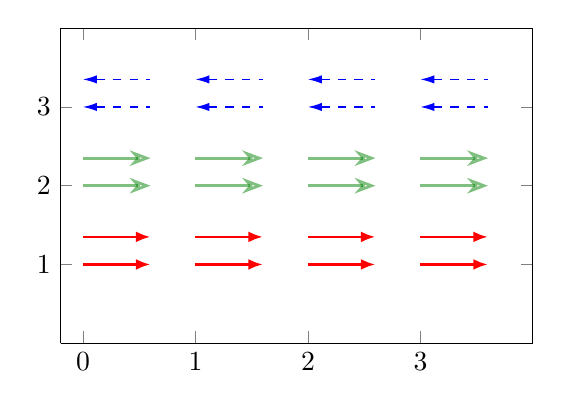
\begin{tikzpicture}
\begin{axis}[view={0}{90},scale only axis,width=6cm,height=4cm,
  xmin=-.2,xmax=4,ymin=0,ymax=4,zmin=-1,zmax=1,enlargelimits=false,
  domain=0:3,samples=4,samples y=2,xtick={0,1,2,3},ytick={1,2,3}]
  \addplot3[blue,y domain=1:1.35,quiver={u=.6,v=0,
    every arrow/.style={-{Latex[scale=.7]},draw=red,line width=1pt}}] {0};
  \addplot3[blue,opacity=.5,y domain=2:2.35,/pgfplots/quiver={u=.6,v=0,
    every arrow/.style={-{Stealth[open]},line width=1pt},
    every arrow/.append style={draw=green!50!black}}] {0};
  \addplot3[blue,y domain=3:3.35,quiver={u=.6,v=0,
    every arrow/.style={{Latex[length=5pt,width=3pt]}-,dashed}}] {0};
\end{axis}
\end{tikzpicture}
\end{document}
